\chapter{Top Quark and Higgs Boson Reconstructions}
\label{Application}

\begin{quote}
\textit{The \tth application for event reconstruction is presented in this chapter. Its dependencies are presented. The flow of the application is presented in section \ref{Application:Flow}, together with a schematic representation. Its main functions are presented and the schematic flow is compared against a callgraph of the application to help understanding what happens in each of the most important functions. The critical region is identified in section \ref{CriticalRegion} and characterized in subsection \ref{ComputationalCharactrization}. Some initial optimizations to the code are presented in subsection \ref{InitialOptimizations}.}
\end{quote}

The LIP research group developed the \tth application to reconstruct the top quark and Higgs boson resultant from a collision, and fits in the Tier-3 grid computational resources. Its name derived from the problem it was design to solve: the \textit{tt} is relative to the reconstruction of the \ttbar system; the \textit{H} is derived from the Higgs boson reconstruction; the \textit{dilep} is the name of the function responsable for the kinematical reconstruction, as it needs two leptons (di-lep) as input.

The application has two main dependencies in external libraries. The first, and most important, is on ROOT \cite{CERN:ROOT}, a object oriented framework, developed at CERN, which provides a set of funcionalities oriented for handling, analysing and displaying results relative to the large amounts of data collected at the LHC. It provides an API for reading and storing data in the standard formats accepted by all the tier centres, classes for representing physic elements, mathematical routines, pseudo-random number generators, histograms, curve fitting minimization and data visualization methods. It was originally designed and developed by physicists, self taught programmers. This results in a framework with room for improvement, such as code restructuring in some modules related to the data analysis that would increase its performance. Other possible optimizations include replacing some mathematical functionalities by using faster libraries, such as BLAS \cite{BLAS} or MKL \cite{MKL}. The Parallel ROOT Facility (PROOF) \cite{CERN:PROOF} is a ROOT extension for data distribution on distributed memory systems.

The second dependency is on the LipMiniAnalysis library. It is a modified version of LipCbrAnalysis, a library developed by LIP for in-house use, which provides a skeleton (not an API) for creating an analysis application. It offers a code structure common for most applications developed by LIP, where the programmer codes specific parts of it depending on the analysis. The current implementation of this library is not suitable for parallelization in shared or distributed memory, as later explained in chapter \ref{ParallelizationApproaches}.

The following sections present the flow of the application and an early profiling, identifying and characterizing the performance bottlenecks.

\section{The \tth application flow}
\label{Application:Flow}

This section describes the workflow of the \tth analysis. The application flow is schematized in figure \ref{fig:SchematicFlow1}. It has two main steps repeated for every event in the input data file: 

\begin{description}
	\item[Load Event Data:] information relative to the event, the bottom quark jets and leptons characteristics, as well as other control data, are loaded to a global state. Most of this state is part of the LipMiniAnalysis and it is over-written every time a new event is loaded. \ttLoop is the function that loads and processes all events.
	\item[Process Event:] most of the event processing is performed in the \ttDoCuts function. This function applies a set of filters to an event (referred as cuts), where it can be rejected if it does not match the criteria of any of the filters. These cuts test many characteristics of the events data, such as the number of isolated leptons with opposite signs, the number of jets and the value of the particles masses. Only the events that reach cut number 20 are fit for the \ttbar system and Higgs boson reconstructions, which are performed in this filter by a complex function named \ttDilepKinFit. From a computational point of view, all the cuts are simple with the exception of cut 20.
	\begin{description}
		\item[\ttDilepKinFit:] this is the function that reconstructs the events. It has an outer loop that iterates through all the possible combinations of 2 bottom quark jets and 2 leptons. Once the combination to process is found an inner loop iterates through the number of variations per combination, defined at compile time. These are the variations of the particle characteristics to improve the reconstruction quality. The next step is to apply the variation to the particles characteristics and then attempt to reconstruct the \ttbar system (kinematical reconstruction). If a reconstruction is possible, the Higgs boson is also reconstructed and the combined probability of the reconstructions is computed. If not, that variation is discarded, as it is not possible to reconstruct the Higgs boson without information relative to the \ttbar system. The probability depends on the accuraccy of the kinematical and Higgs boson reconstructions. Most of the handled data by this cut is stored in the global state of LipMiniAnalysis.
	\end{description}
\end{description}

\begin{figure}[!htp]
	\begin{center}
		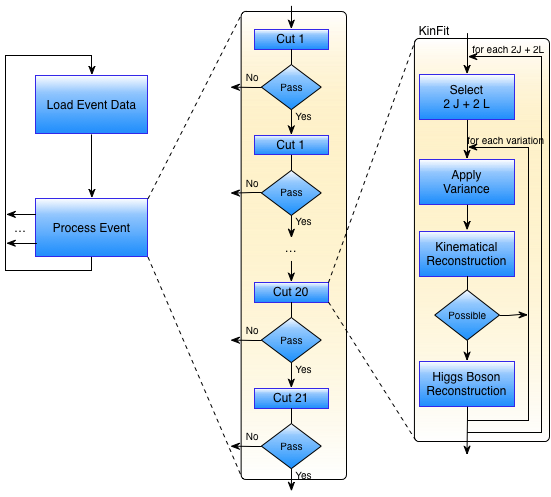
\includegraphics[scale=0.6]{../../common/img/graf_abstract_flow_with_kinfit.png}
		\caption{Schematic representation for the \tth application flow.}
		\label{fig:SchematicFlow1}
	\end{center}
\end{figure}

This schematic representation of the application flow was designed based on the source code and the callgraphs analysis, obtained by using the callgrind tool from Valgrind \cite{Valgrind}. Besides giving an inside of the application structure, this tool provides simple profiling information, measuring how much percentage of time is spent in each function, for a rough assement of the possible bottlenecks. The callgraph for the application\footnote{See appendix \ref{App:TestEnv} for characterization of all the used systems.} is presented in figure \ref{fig:Callgraph1} and, since the goal is to run as many variations per combination within a reasonable time frame, as explained in section \ref{Motivation}, a callgraph for 256 variations per combination is presented in figure \ref{fig:Callgraph256}. Note that only the relevant functions are included in the callgraphs below, as the complete callgraph is much larger.

\begin{figure}[!htp]
	\begin{center}
		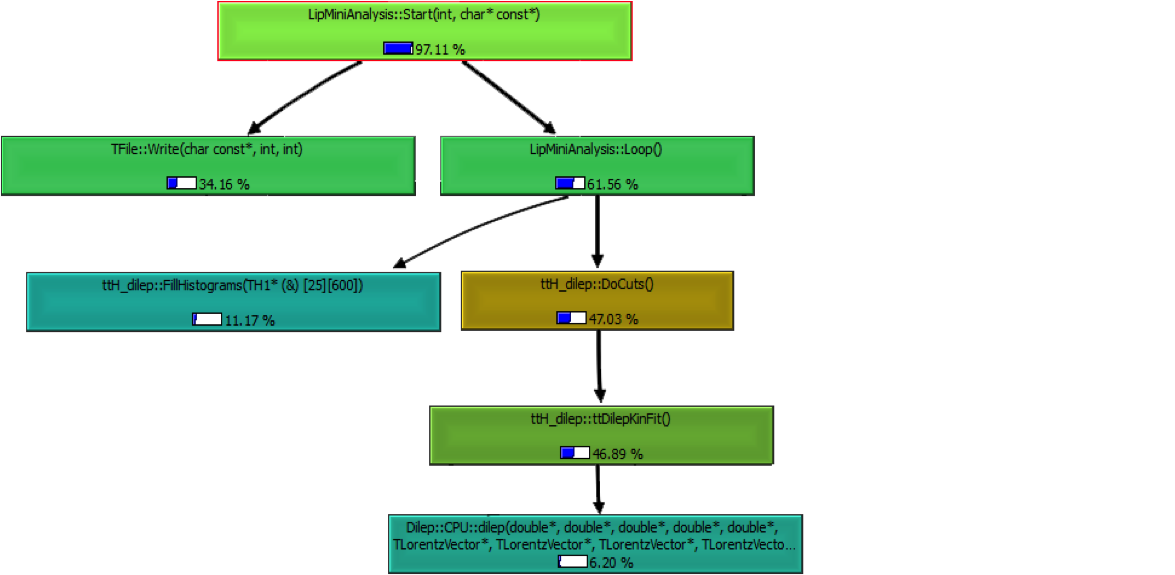
\includegraphics[scale=0.7]{../../common/img/callgraph_start_1.png}
		\caption{Callgraph for the \tth application on the compute-711 node.}
		\label{fig:Callgraph1}
	\end{center}
\end{figure}

\begin{figure}[!htp]
	\begin{center}
		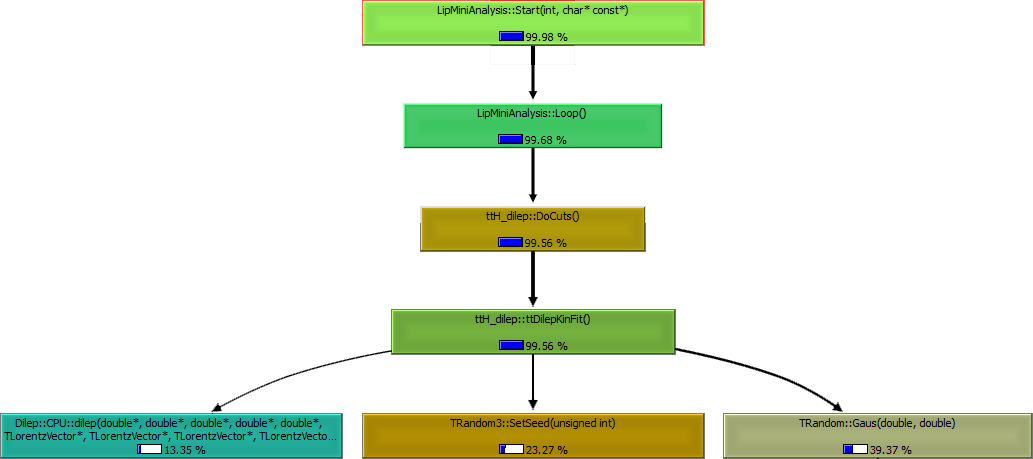
\includegraphics[scale=0.7]{../../common/img/callgraph_start_256.png}
		\caption{Callgraph for the \tth application on the compute-711 node for 256 variations per combination.}
		\label{fig:Callgraph256}
	\end{center}
\end{figure}

When not performing variations, a third of the execution time is spent in writing outputs to files, using the ROOT library (note that all classes with a capital \textit{T} as prefix belong to ROOT) and the rest is spent processing the events. The cut number 20, \ttDilepKinFit, takes most of the event processing time, where 6.2\% of the time is on the kinematical reconstruction (\dilep). It is clear that this cut is the portion of the application that uses most of the event processing time. This becomes even more evident when considering 256 variations per event, where \ttDilepKinFit uses 99.6\% of the application execution time.

For a high number of variations of the input parameters, it is clear that the pseudo-random number generator (\texttt{TRandom} and \texttt{TRandom3} classes) is taking a substantial part of the cut execution. Table \ref{tab:TempoKinFit} shows the percentage of the application execution time spent on \ttDilepKinFit, for various variations per combination. In section \ref{CriticalRegion} a computational analysis of the critical region is presented, as well as some early optimizations to the application.

\begin{table}[!htp]
	\begin{center}
		\begin{tabular}{|c|c|c|c|c|c|c|c|c|c|c|}
			\hline
			\textbf{\# of variations/combination} & 1 & 2 & 4 & 8 & 16 & 32 & 64 & 128 & 256 & 512 \\ \hline
			\textbf{\% of time} & 46.9 & 62 & 76.9 & 87 & 92.9 & 96.3 & 98 & 98.9 & 99.6 & 99.7 \\ \hline
		\end{tabular}
		\caption{Percentage of the total execution time spent on the \ttDilepKinFit function for various numbers of variations per combination.}
		\label{tab:TempoKinFit}
	\end{center}
\end{table}

\section{The computing critical region}
\label{CriticalRegion}

This section focus on the computational characterization of the \ttDilepKinFit function. It analyses in terms of instruction mix, the arithmetic and computational intensity and the miss rate, aiming to understand how this region of the code behaves, for various variations per combination, and classify it as a memory or compute bound algorithm. The testbed system used in this section is the compute-711\footnote{See appendix \ref{App:TestEnv} for characterization of all the systems used.}. Some initial optimizations, as well as other changes made to the original application, will be addressed in section \ref{InitialOptimizations}.

\subsection{Computational characterization}
\label{ComputationalCharactrization}

The \ttDilepKinFit, often referred as KinFit, is the most time consuming task in \tth application. Figure \ref{fig:KinFitGraph} shows the evolution of the absolute and relative execution time of the KinFit function and the I/O of the application, which was also identified by callgraph \ref{fig:Callgraph1} as a time consuming task for a low number of variations, and the remaining computations.

\begin{figure}[!htp]
	\begin{center}
		\raisebox{-0.5\height}{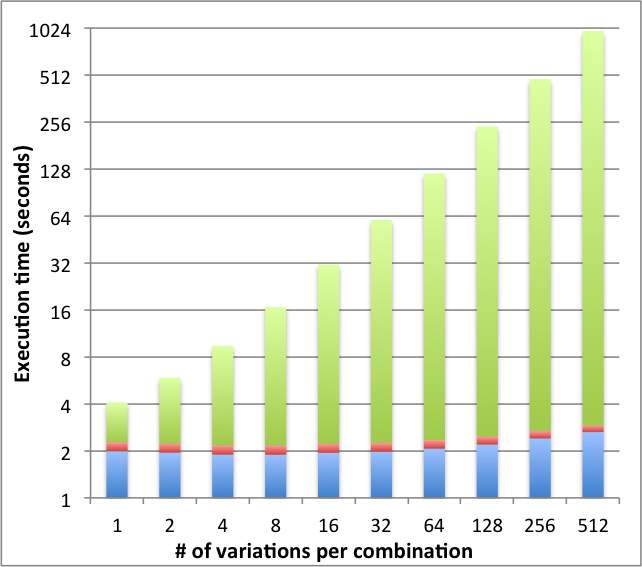
\includegraphics[scale=0.6]{../../common/graphs/exec_time_kinfit_rest.png}}
		\raisebox{-0.5\height}{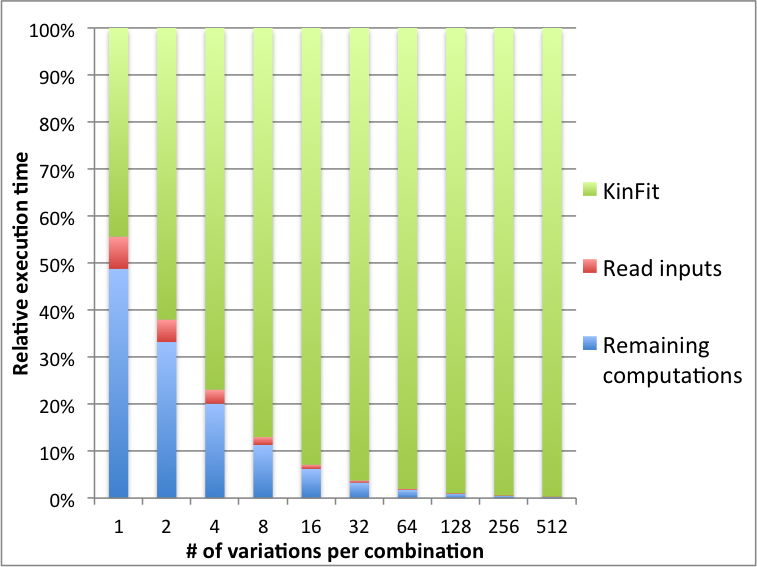
\includegraphics[scale=0.6]{../../common/graphs/relative_exec_time_kinfit_rest.png}}
		\caption{Absolute (left) and relative (right) execution times for the \tth application considering the \ttDilepKinFit (KinFit) function, I/O and the rest of the computations.}
		\label{fig:KinFitGraph}
	\end{center}
\end{figure}

The I/O and the event processing execution times, excluding the KinFit, remain constant. There is only a slight increase for 256 and 512 variations as it causes more events to be reconstructed, which otherwise would not, and pass to the final cut 21 (see figure \ref{fig:SchematicFlow1}). As expected, the execution time of KinFit linearly increases with the number of variations per combination. This indicates that the arithmetic intensity of KinFit has the complexity of \textit{O(N)}, where \textit{N} is the number of variations. Consider a given input data file. With no variations, it is possible to consider that the time to process the events remains constant as long as the application is executed, while using the given input data file. This is the initial problem size. The increase in variations, causing the number of reconstructions to grow linearly, is responsible for the increase in the problem size. So, for \textit{N} variations it is expected that KinFit execution time will increase by the same factor. This analysis is supported by the experimental data in figure \ref{fig:KinFitGraph}, left graph.

\begin{figure}[!htp]
	\begin{center}
		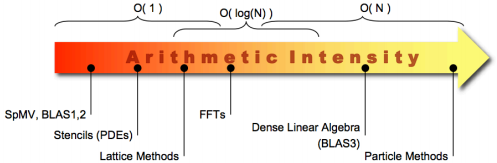
\includegraphics[scale=0.6]{../../common/img/arithmetic_intensity.png}  
		\caption{Arithmetic intensity for various domains of computing problems.}
		\label{fig:ArithmeticIntensity}
	\end{center}
\end{figure}

Figure \ref{fig:ArithmeticIntensity} presents the complexity for various computational purposes. Problems with \textit{O(1)} complexity are not likely to get any benefit from parallelization, opposed to problems with \textit{O(N)} complexity, which are more easy to be efficiently parallelized.

For the rest of the computational characterization, the \ttDilepKinFit function was analysed resorting to hardware performance counters, using the Performance API, PAPI \cite{PAPI}. The application was tested on the compute-601 system for various numbers of variations per combination. The instruction mix is presented in figure \ref{fig:InstMix}. It is evident, by analysing the charts, that the performance of this function cannot be evaluated using the common FLOPS metric, as float point operations only account for 14\% and 12\% of the total instructions, for 1 and 512 variations respectively. \ttDilepKinFit is very diverse in terms of instructions, with loads, branches and stores being the most used. The increase in the number of variations does not have a significant impact on the type of issued instructions.

\begin{figure}[!htp]
	\begin{center}
		\raisebox{-0.5\height}{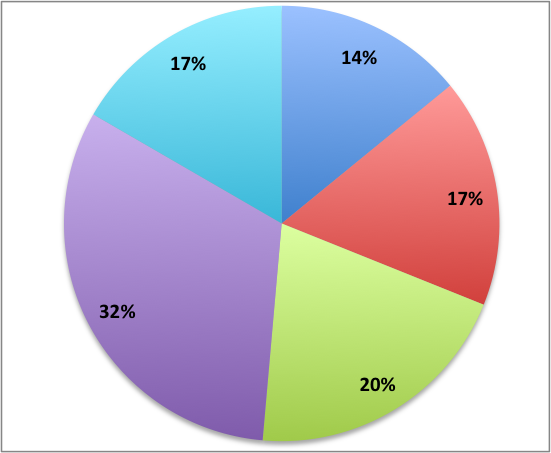
\includegraphics[scale=0.7]{../../common/graphs/inst_mix.png}}
		\raisebox{-0.5\height}{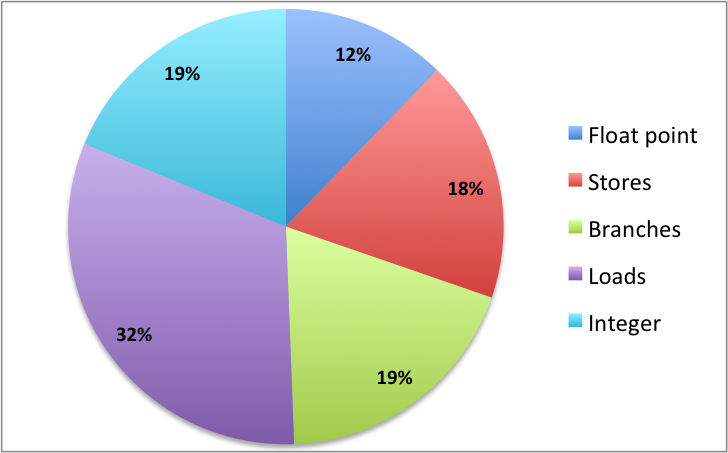
\includegraphics[scale=0.7]{../../common/graphs/inst_mix_256.png}}
		\caption{Instruction mix for the \ttDilepKinFit with no and 512 variations, left and right images respectively.}
		\label{fig:InstMix}
	\end{center}
\end{figure}

The miss rate, for the 3 cache levels, is presented in figure \ref{fig:MissRate}. The miss rate on L1 cache remains constant at 70\%, despite the change in variations. Even though this value is high, it is justified by the large amount of different computations required to reconstruct an event, where data is only reused between subsequent instructions (considering the scope of the small L1 cache size), rather than periodically reused. The L2 cache miss rate is fairly low and decreases with the number of variations. As it has a larger size than L1 cache, the data is reused more often without causing misses to the L3 cache. Due to the reuse of data in the L2 cache, and considering the larger size of the L3 cache, the miss rate on the last cache level increases with the number of variations. This is not a consequence of a deficient cache management, but results from the decrease of the L2 cache miss rate, where most L2 cache misses are due to the need to access new data on RAM. The use of more cores, in a shared memory environment, may result in a decrease in the miss rate, specially on L2 cache, as each core will process a smaller data set.

\begin{figure}[!htp]
	\begin{center}
		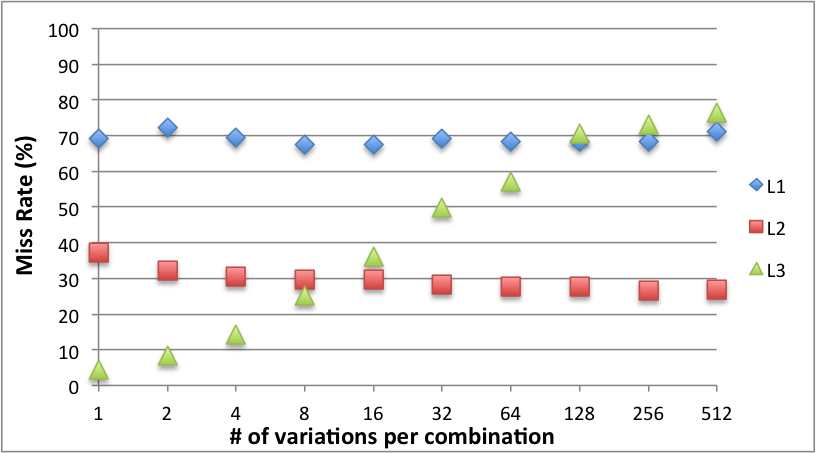
\includegraphics[scale=0.8]{../../common/graphs/miss_rate.png}  
		\caption{Miss rate on L1, L2 and L3 cache of \ttDilepKinFit for various number of variations.}
		\label{fig:MissRate}
	\end{center}
\end{figure}

Operational intensity \cite{Roofline} is a performance metric used to characterize the bottlenecks of a given algorithm, based on the assumption that accesses to the system RAM memory are the main performance limitation on current systems. It allows classifying an algorithm as memory or compute bound, depending on which factor limits its performance. It requires a Roofline model\footnote{Roofline model for the test system is presented and explained in appendix \ref{App:Roofline}.} for the system in which the operational intensity is computed. The operational intensity is defined by the amount of float point operations performed per each byte of data fetch from the system RAM memory. However, this is not a reliable metric for this specific problem as only 17\% of the instructions of \ttDilepKinFit are float point arithmetic (refer to chart \ref{fig:InstMix}). Instead, the computational intensity is considered a more reliable metric if it includes all kinds of instructions, with the exception of load and store instructions, which are not relevant for the algorithm structure.

\begin{figure}[!htp]
	\begin{center}
		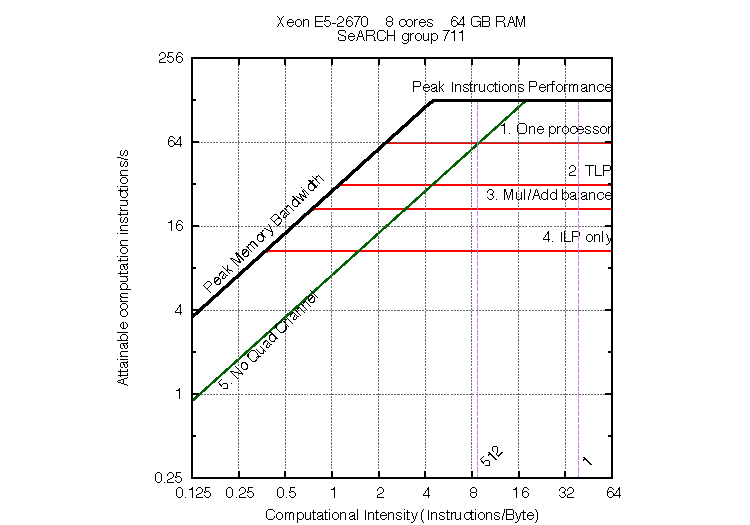
\includegraphics[scale=1]{../../common/601_papi.pdf}  
		\caption{Roofline of the compute-601 system with the computational intensity of \ttDilepKinFit for 1 and 512 variations.}
		\label{fig:Roofline}
	\end{center}
\end{figure}

Figure \ref{fig:Roofline} presents the Roofline model for the compute-601 system with the computational intensity for \ttDilepKinFit with 1 and 512 variations. For both number of variations it is obvious that this is a compute bound problem, only limited by the peak computational performance of the CPU. For 512 variations the computational intensity is lower than for 1 variation, however the \ttDilepKinFit execution time still increases linearly, as shown in figure \ref{fig:KinFitGraph}, because it is still only limited by the CPU roofline. More of the CPU resources are being used to keep up with the linear increase in time, relatively to 1 variation that underuses the said resources. This indicates that the optimizations must be focused on increasing the computational throughput rather than on RAM memory access patterns. Note that cache optimizations are related to the computational throughput.

\subsection{Initial optimizations}
\label{InitialOptimizations}

One limiting factor for the \ttDilepKinFit function is the pseudo-random number generation (PRNG) performed by the \texttt{TRandom} ROOT class, specifically when performing a high number of variations, as seen in callgraph \ref{fig:Callgraph256}. When applying a variation to a combination in the \ttDilepKinFit function, 12 PRNG values are needed at most. After generating the uniformly distributed numbers, a transformation is applied on them so that they obey a Gaussian distribution. The number is generated and transformed by the \texttt{Gauss} function, which occupies 39.4\% of the total execution time. In the input data file used\footnote{See Appendix \ref{App:TestMethodology} for a complete characterization of the test methodology.}, 1867 events reach the cut 20. This means that 244056 combinations are varied, with a total of 2928672 values generated for just a single variation per combination. This is also likely to happen with other input data files as they hold a similar number of events. In the \ttDilepKinFit surce code, the \texttt{TRandom} generator is being reset with a new seed for every combination, causing 23.4\% of execution time to be spent on the \texttt{SetSeed} function.

The pseudo-random number generator used by the \texttt{TRandom3} class is the Mersenne Twister \cite{MersenneTwister}, currently one of the most used generators for applications highly dependable on pseudo-random numbers. This algorithm produces 32-bit uniformly distributed pseudo-random numbers with a period of $2^{19937}$. It has a relatively heavy state which is an integrant part on the algorithm flow. The generator is thread safe as long as different states are being used by different threads. The state can be shared among the threads but, modifying it must be serialized, and the generated number by one thread will affect the other generated numbers. A proper implementation of this generator for a parallel algorithm must use one state per thread.

Since the period of the Mersenne Twister is $2^{19937}$ (approximately $4.3 * 10^{6001}$) and the maximum amount of generated numbers in the test file used, for 512 variations per combination, is $1.5 * 10^{9}$, it is not necessary to reset the seed of the \texttt{TRandom3} generator for every combination, which can significantly reduce the \ttDilepKinFit execution time. Figure \ref{fig:TRandomOptim} illustrates the speedup obtained through this optimization. For a larger number of variations (from 16 to 512) the application is 1.7 to almost 2 times faster, without affecting the quality of the results.

\begin{figure}[!htp]
	\begin{center}
		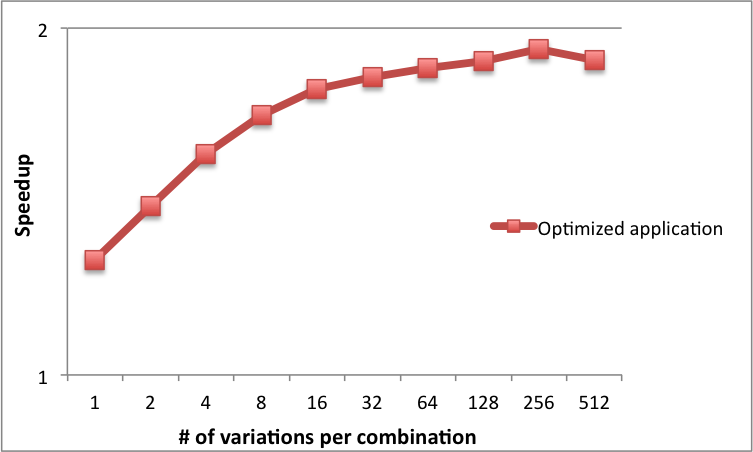
\includegraphics[scale=0.7]{../../common/graphs/speedup_trandom_optim.png}  
		\caption{Speedup of the \tth application with the \texttt{TRandom} optimization.}
		\label{fig:TRandomOptim}
	\end{center}
\end{figure}

\nvidia offers, in the cuRand library \cite{NVIDIA:cuRand}, a parallel implementation of the Mersenne Twister for GPUs \cite{NVIDIA:MersenneTwister}, which is relevant to port the critical region to run on heterogenous systems with this hardware accelerator. It uses a precomputed set of 200 parameters, which can also be generated by the user, for the configuration of the generator's state, but offering a smaller period of $2^{11213}$. The pseudo-random number generation is thread safe, allowing up to 256 threads sharing the same state per block. Two different blocks can safely operate concurrently on the same SM.

\texttt{TRandom} uses the Acceptance-Complement Ratio algorithm \cite{AcceptanceRandom} for transforming the pseudo-random numbers from an uniform to a gaussian transformation. It is allegely 66\% faster than the Box-Muller transformation \cite{BoxMuller} and similar in performance to the Ziggurat method \cite{Ziggurat}. The cuRand library only offers the Box-Muller transformation with a basic pseudo-random number generator so, to accuratly replicate the results, it is needed to replicate the \texttt{TRandom} gaussian method on GPU using the cuRand implementation of Mersenne Twister.

Other modifications were made to the application, structuring the computation of the variations and kinematical reconstruction in modules, in such a way that when developing different parallel versions of \ttDilepKinFit it is easy to switch between them, and also increasing code readability. The definition of the number of variations to perform is set by environment variables, at runtime, rather than at compile time, as it is on the original application, easing the user interaction.
